\section{Цель работы}
Для заданного объекта управления синтезировать оптимальное управление, при заданных критерии качества, начальных условиях и ограничениях  (принцип максимума).



\section{Теоретические сведения}
Рассматриваемый объект управления:
\begin{equation}\label{system}
	\dot{x} = a x + b u, \quad x(0)
\end{equation}
где $a$, $b$~--- известные параметры. 

Критерий качества для системы~\eqref{system} с фиксированным временем и фиксированными концами:
\begin{equation}
	J_A = \int\limits_0^{t_f} H(x,u,\lambda) + \dot\lambda x d \tau + \theta \eta_2 (x(t_f))
\end{equation}
где $H(x,u,\lambda) = L(x,u) + \lambda f(x,u)$, $\theta$~--- множитель Лагранжа (константа), $\eta_2$~--- функция для фиксации положения в $t_f$. 

Функция накладывающая ограничение на значение состояния ОУ в момент времени~$t_f$:
\begin{equation}
	\eta_2 (x(t_f)) = x(t_f) - x_f = x(t) \bigl|_{t = t_f} - x_f
\end{equation}

Уравнение оптимальности:
\begin{equation}
	\cfrac{\partial H}{\partial u} = 0
\end{equation}

Уравнение сопряженной системы:
\begin{equation}
	\dot\lambda = - \cfrac{\partial H}{\partial x}
\end{equation}

Уравнение трансверсальности:
\begin{equation}
	\Biggl( - \lambda + \theta \cfrac{\partial \eta_2}{\partial x} \Biggr) \Biggl|_{t_f}  = 0
\end{equation}


\section{Исходные данные}
Варианту \textnumero2 соответствует следующий набор исходных данных:
\begin{equation}\label{init}
	\dot x = -2 x + u,
	\quad
	J = \int\limits_{0}^{1} x^2(\tau) + u^2(\tau)\, d\tau,
	\quad
	x(1) = 5 \ldotp
\end{equation}


\section{Результаты практических действий}

Запишем Лагранжиан и Гамильтониан системы:
\begin{equation}
	L(x,u) = x^2 + u^2,
	\quad
	H(x,u,\lambda) = x^2 + u^2 + \lambda (-2 x + u)
\end{equation}

Найдем структуру регулятора из уравнения оптимальности:
\begin{equation}
	2u + \lambda = 0
	\quad\Rightarrow\quad
	u = -\cfrac{1}{2} \lambda
\end{equation}

Тогда ОУ:
\begin{equation}
	\dot x = -2 x - \frac{1}{2}\lambda
\end{equation}

Запишем уравнение сопряженной системы:
\begin{equation}
	\dot\lambda = 2 \lambda - 2 x
\end{equation}

Объединим модели ОУ с регулятором и сопряженной системы и запишем:
\begin{equation}
	\begin{aligned}
		& \dot{x} = - 2 x - \frac{1}{2} \lambda \\
		& \dot \lambda = -2 x + 2 \lambda
	\end{aligned}
	\quad\Rightarrow\quad
	\dot \xi = A_{\xi} \xi
	\quad\Rightarrow\quad
	\xi = e^{A_\xi t} \xi(0)
\end{equation}
где $\xi = \begin{bmatrix}x & \lambda\end{bmatrix}^T\!\!$, $A_{\xi} = \begin{bmatrix}-2 & -\frac{1}{2} \\-2 & 2\end{bmatrix}\!$.

Из условия трансверсальности:
\begin{equation}
	\lambda(t_f) = \theta
\end{equation}

И, используя заданные ограничения, получим:
\begin{equation}
	\xi(1) = e^{A_\xi} \xi(0)
	\quad\Leftrightarrow\quad
	\begin{bmatrix}
		5\\
		\theta
	\end{bmatrix}
	= Z
	\cdot
	\begin{bmatrix}
		x(0) \\
		\lambda(0)
	\end{bmatrix}
	\quad\Rightarrow\quad
	\lambda(0) = \cfrac{5 - Z_{11} x(0)}{Z_{12}}
\end{equation}
где $Z = e^{A_\xi}$.

\begin{table}[h!]
	\centering
	\caption{Значения критерия качества для различных начальных условий и различных коэффициентах регулятора}
	\label{criteries}
\begin{tabular}{|r|c|c|c|}
	\hline
	\multicolumn{1}{|l|}{\cellcolor{}} & \begin{tabular}[c]{@{}c@{}}Опт. регулятор\\ u = - 0.5 \lambda\end{tabular} & \begin{tabular}[c]{@{}c@{}}Неоптимальный\\ u = -0.1 \lambda\end{tabular} & \begin{tabular}[c]{@{}c@{}}Неоптимальный\\ u = - 2 \lambda\end{tabular} \\ \hline
	\begin{tabular}[c]{@{}r@{}}J(1.2)\\ x(0)=0\end{tabular} & 107.197 & 107.325 & 108.387 \\ \hline
	\begin{tabular}[c]{@{}r@{}}J(1.2)\\ x(0)=10\end{tabular} & 87.623 & 88.643 & 96.741 \\ \hline
\end{tabular}
\end{table}

Графики переходных процессов показаны на рисунках~\ref{img_graphs_0}--\ref{img_graphs_10}, а использованная дли их получения схема моделирования~--- на рисунке~\ref{img_modeling_scheme}.

\begin{figure}[h!]
    \centering
    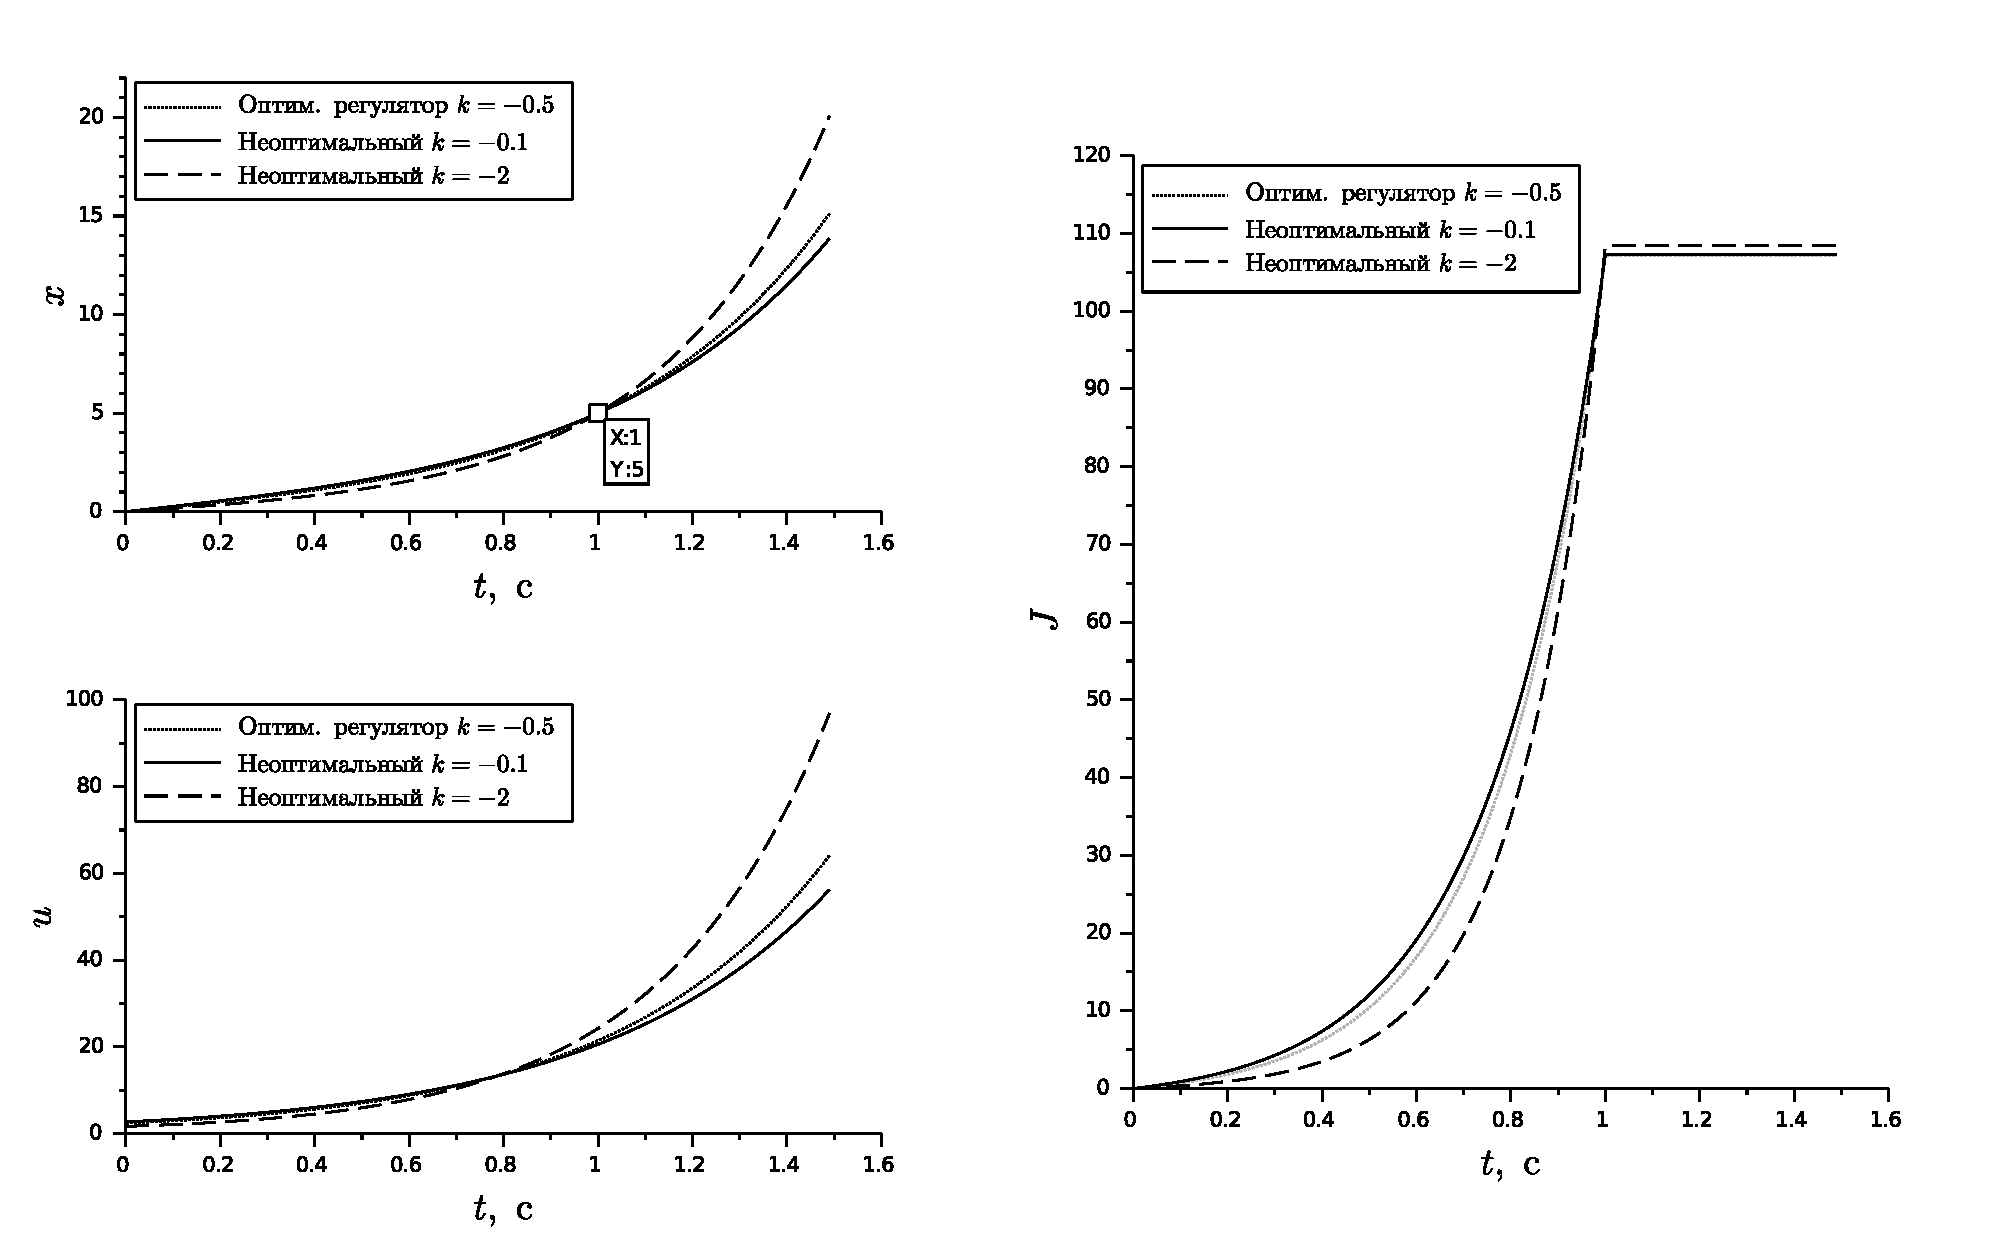
\includegraphics[width=\textwidth]{graphs_x0_0.pdf}
    \vspace{0cm}
    \caption{Графики переходных процессов для начального условия $x(0) = 0$}
    \label{img_graphs_0}
\end{figure}

\begin{figure}[h!]
    \centering
    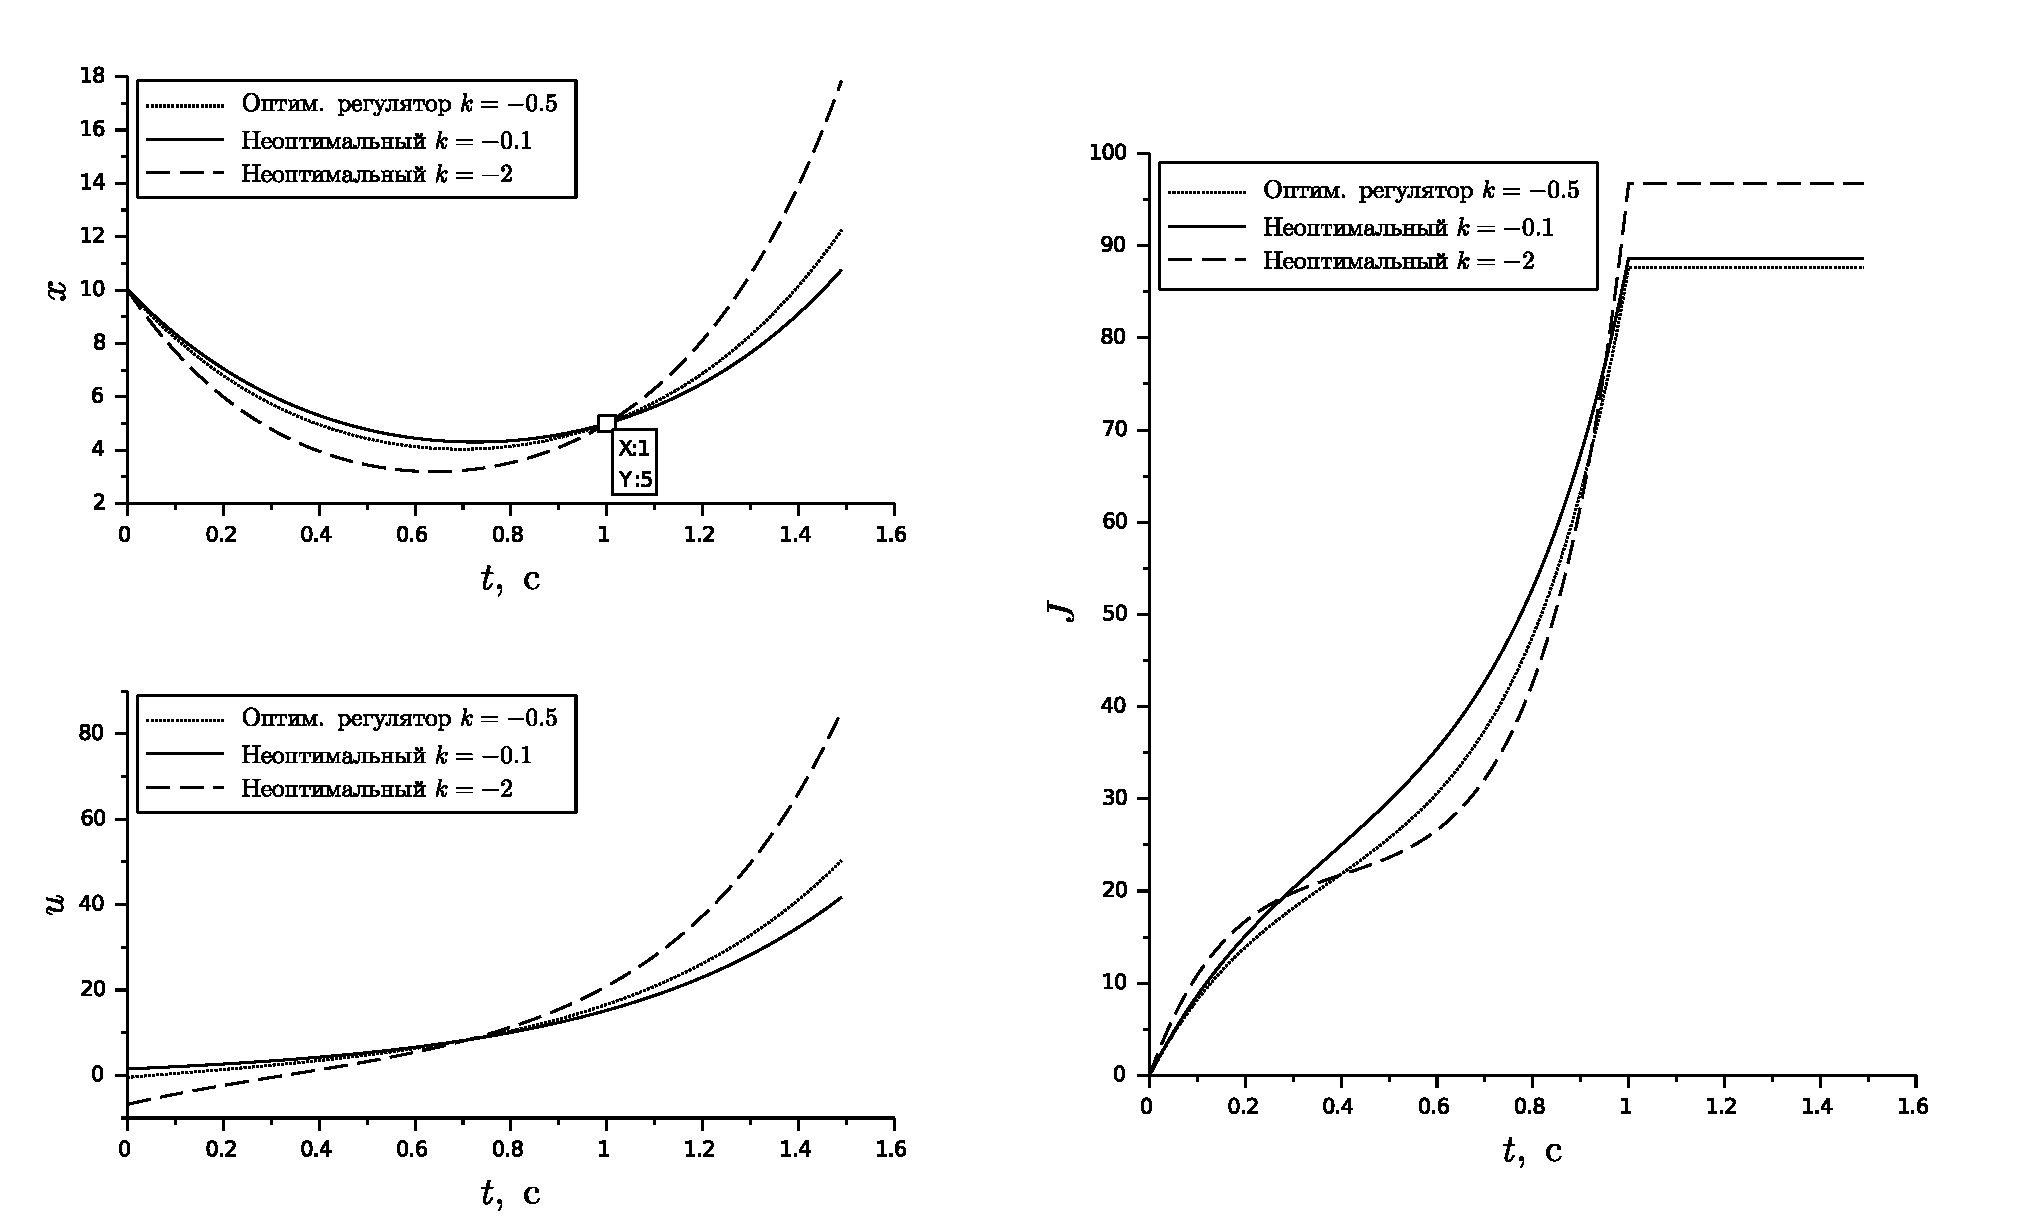
\includegraphics[width=\textwidth]{graphs_x0_10.pdf}
    \vspace{0cm}
    \caption{Графики переходных процессов для начального условия $x(0) = 10$}
    \label{img_graphs_10}
\end{figure}

\clearpage

\begin{figure}[h!]
    \centering
    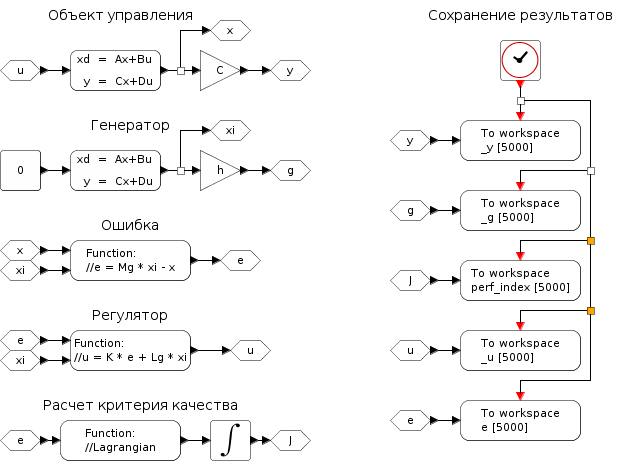
\includegraphics[width=0.9\textwidth]{modeling_scheme.png}
    \vspace{0.5cm}
    \caption{Схема моделирования рассматриваемой системы}
    \label{img_modeling_scheme}
\end{figure}


\section{Выводы по работе}
В~результате проделанной работы для заданного ОУ было рассчитано управление, оптимальным образом решающее задачу управления в условиях наложенного ограничения с точки зрения минимизации критерия~\eqref{init}. 